% ====================================================================================
\begin{frame}
\frametitle{1968 - Cornell's Program of Computer Graphics (PCG)}

\begin{columns}

    % Image on the left
    \begin{column}{0.48\textwidth}
        \centering
        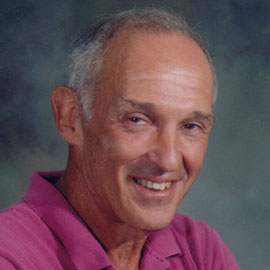
\includegraphics[width=\linewidth]{assets/Greenberg.jpg}
    \end{column}

    % Text on the right
    \begin{column}{0.48\textwidth}
        In 1968, Donald Greenberg joined Cornell University with a joint appointment in architecture and structural engineering. He established the Program of Computer Graphics, helping establish Cornell as an important center for computer graphics.
    \end{column}

\end{columns}

\end{frame}

% ====================================================================================

\begin{frame}
\frametitle{1968 - Evans and Sutherland (E&S)}

\begin{columns}

    % Image on the left
    \begin{column}{0.48\textwidth}
        \centering
        
\includegraphics[width=\linewidth]{assets/ES.png}
    \end{column}

    % Text on the right
    \begin{column}{0.48\textwidth}
        In 1968, David Evans joined the University of Utah and invited Ivan Sutherland to join him, creating an important computer graphics research group. Frustrated by the limited graphics hardware available, Evans and Sutherland founded Evans & Sutherland, one of the first companies dedicated to computer graphics.
    \end{column}

\end{columns}

\end{frame}

%====================================================================================

\begin{frame}
\frametitle{1968 - Foundation of Intel}

\begin{columns}

    % Image on the left
    \begin{column}{0.48\textwidth}
        \centering
        
\includegraphics[width=\linewidth]{assets/Intel_Logo.png}
    \end{column}

    % Text on the right
    \begin{column}{0.48\textwidth}
        In 1968, Robert Noyce and Gordon Moore founded Intel (Integrated Electronics) after leaving Fairchild Semiconductor. The company was established with a strong focus on continuous innovation and research and development, becoming a major force in the development of microprocessors and hardware.
    \end{column}

\end{columns}

\end{frame}

%====================================================================================

\begin{frame}
\frametitle{1968 - Ray-Casting}

\begin{columns}

    % Image on the left
    \begin{column}{0.48\textwidth}
        \centering
        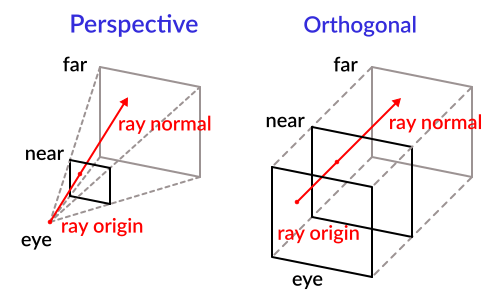
\includegraphics[width=\linewidth]{assets/raycast.png}
    \end{column}

    % Text on the right
    \begin{column}{0.48\textwidth}
        In 1968, Arthur Appel introduced the ray-casting technique to determine surface visibility in computer-generated scenes, and precursor of ray-tracing. The method casts rays from the viewer through each pixel and identifies the closest object intersected, while additional rays determine if the visible point is in shadow.
    \end{column}

\end{columns}

\end{frame}
